\documentclass{article}

\usepackage{parskip}
\usepackage[T1]{fontenc}
\usepackage[a4paper, total={6in, 8in}]{geometry}
\usepackage[scale=.97]{sourcecodepro}
\usepackage{titlesec}
\usepackage{tikz}
\usepackage{listings}
\usetikzlibrary{arrows.meta,chains,decorations.pathreplacing}
\usepackage{xcolor}

\newcommand{\code}[1]{\lstinline[language=C]!#1!}

%New colors defined below
\definecolor{codegreen}{rgb}{0,0.6,0}
\definecolor{codegray}{rgb}{0.5,0.5,0.5}
\definecolor{codepurple}{rgb}{0.58,0,0.82}
\definecolor{backcolour}{rgb}{0.95,0.95,0.92}

%Code listing style named "mystyle"
\lstdefinestyle{mystyle}{
  backgroundcolor=\color{backcolour},   commentstyle=\color{codegreen},
  keywordstyle=\color{magenta},
  numberstyle=\tiny\color{codegray},
  stringstyle=\color{codepurple},
  basicstyle=\ttfamily\footnotesize,
  breakatwhitespace=false,         
  breaklines=true,                 
  captionpos=b,                    
  keepspaces=true,                 
  numbers=left,                    
  numbersep=5pt,                  
  showspaces=false,                
  showstringspaces=false,
  showtabs=false,                  
  tabsize=2
}

\lstset{style=mystyle}

\title{CPS1011 - Programming Principles in C}
\author{Giorgio Grigolo}
\date{Semester 1 - 2021/22}


% \titleformat{\section}
% 	{\scshape}{\thesection}{1em}{}
\titleformat{\section}[block] % section
  {\Large\scshape}
  {}
  {0pt}{\filcenter}[]
\titlespacing*{\section}
  {0em} %left
  {0em} %before
  {2em} %after

\begin{document}

	\maketitle
	\tableofcontents
	\newpage

	\section{Task 1 - Problem Solving}

	\subsection{Header File}

	\lstinputlisting[language=C, firstline=1, lastline=10]{task1/task1.h}

	\subsection{Function Definitions}
	\subsubsection{\texttt{init\_array()}}
		
	\lstinputlisting[language=C, firstline=60, lastline=82]{task1/task1.c}

	The above function iterates indefinitely, until a valid input is obtained for the length of the
	array to be initialized. Furthermore, it will iterate for as many times as was previously entered
	by the user, whilst requesting further input to populate the array specified in the function
	parameter \code{int *input_array}.

	The \code{while} loop from lines 7-13 performs a \textbf{bitwise or} on the
	range check ensuring that the input is an integer such that $0 < \texttt{length} \leq 200$. 
	An extremal bound check is performed in the \code{if} statement in lines 10-12 to alert the user
	about erroneous input in case the above restrictions are ignored.

	A \code{for} loop is used in lines 15-18 to ask the user \code{length} times for an input which is
	stored in the location pointed to by the address stored in \code{input_array[i]}.

	Finally, it returns the length specified by the user as an integer, to be later used in other functions.


	\newpage
	 
	\subsubsection{\texttt{display()}}

	\lstinputlisting[language=C, firstline=84, lastline=98]{task1/task1.c}

	The above function simply displays any integer array passed to it, specifically in the \textbf{JSON}
	format, given that its size is also passed to the function. 

	Firstly, the \code{clear_term()}\footnote{This will be analyzed later, in the \textbf{Utility
	Function Definitions} subsection.} function is run to clear the terminal in preparation of the
	following output. In lines 3 and 14, the JSON header and footers are printed, which are
	independent from any data within. The notation \code{printf(\%*s, n, "foo")} prints the string
	\code{"foo"} for \code{n} times consecutively. As such, it is used to have a fixed tab
	representation\footnote{Tab representations may vary, and thus we ensure the convention of
	1 tab = 4 spaces.}, regardless of environment or operating system.

	Lines 4-13 contain a \code{for} loop which iterates through the array passed as \code{int 
	*input_array} and prints a block of 4 lines with the help \code{jprintf()}\footnotemark[1] as
	follows: 

	\begin{enumerate}
		\item 8 spaces followed by a \code{"\{"},
		\item a JSON entry with attribute name \code{"offset"} and its value stored in \code{i},
		\item a JSON entry with attribute name \code{"value"} and its value stored in the address
			pointed to by \code{input_array[i]}
		\item 8 spaces followed by a \code{"\}"} and a \code{","} only if the current iteration is not the last one.
	\end{enumerate}

	It is to be noted that each of these blocks represents one element in the \code{int *initial_array}.

	\newpage

	\subsubsection{\texttt{reverse()}}

	\lstinputlisting[language=C, firstline=100, lastline=109]{task1/task1.c}

	This function accepts two arrays containing pointers pointing to integers and their length. It is
	worth noting that since \code{array_a} is read-only, it has been declared as \code{const int
	*array_a}, i.e. constant.

	In essence, the \code{while} loop that spans lines 4-8 iteratively sets the first element of
	\code{array_b} equal to the last element of \code{array_a} (line 5), then the second element of
	\code{array_b} equal to the second to last element of \code{array_b} and so on, until the counter
	\code{end} reaches 0. 

	Particularly, this is achieved by keeping track of the offsets for the two arrays stored inside the
	local variables \code{start} and \code{end} by incrementing the first, whilst decrementing the
	second.

	Below is a block-view of an arbitrary run of the \code{reverse()} function, where \code{length} = 4.

	\vspace{3em}

\begin{center}
	{\large \texttt{array\_a} \hspace{7em} \texttt{array\_b}}
\end{center}

\vspace{1em}

\begin{center}
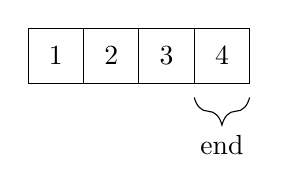
\begin{tikzpicture}[start chain = going right, node distance = 0pt, MyStyle/.style={draw, minimum width=2em, minimum height=2em, outer sep=0pt, on chain}]
	\node [MyStyle] (1) {$1$};
	\node [MyStyle] (2) {$2$};
	\node [MyStyle] (3) {$3$};
	\node [MyStyle] (4) {$4$};
	\draw[decorate,decoration={brace, amplitude=10pt, raise=5pt, mirror}] (4.south west) to node[black,midway,below= 15pt] {\code{end}} (4.south east);%
\end{tikzpicture}
\hspace{5em}
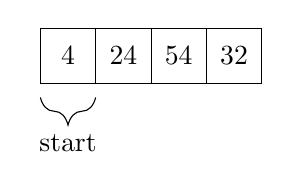
\begin{tikzpicture}[start chain = going right, node distance = 0pt, MyStyle/.style={draw, minimum width=2em, minimum height=2em, outer sep=0pt, on chain},  ]
	\node [MyStyle] (1) {$4$};
	\node [MyStyle] (2) {$24$};
	\node [MyStyle] (3) {$54$};
	\node [MyStyle] (4) {$32$};
	\draw[decorate,decoration={brace, amplitude=10pt, raise=5pt, mirror}] (1.south west) to node[black,midway,below= 15pt] {\code{start}} (1.south east);%
\end{tikzpicture}
\end{center}
\begin{center}
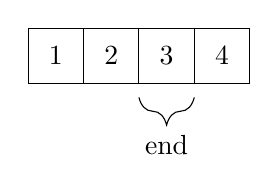
\begin{tikzpicture}[start chain = going right, node distance = 0pt, MyStyle/.style={draw, minimum width=2em, minimum height=2em, outer sep=0pt, on chain}]
	\node [MyStyle] (1) {$1$};
	\node [MyStyle] (2) {$2$};
	\node [MyStyle] (3) {$3$};
	\node [MyStyle] (4) {$4$};
	\draw[decorate,decoration={brace, amplitude=10pt, raise=5pt, mirror}] (3.south west) to node[black,midway,below= 15pt] {\code{end}} (3.south east);%
\end{tikzpicture}
\hspace{5em}
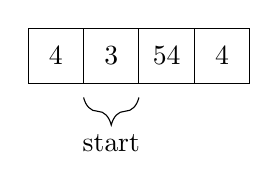
\begin{tikzpicture}[start chain = going right, node distance = 0pt, MyStyle/.style={draw, minimum width=2em, minimum height=2em, outer sep=0pt, on chain},  ]
	\node [MyStyle] (1) {$4$};
	\node [MyStyle] (2) {$3$};
	\node [MyStyle] (3) {$54$};
	\node [MyStyle] (4) {$4$};
	\draw[decorate,decoration={brace, amplitude=10pt, raise=5pt, mirror}] (2.south west) to node[black,midway,below= 15pt] {\code{start}} (2.south east);%
\end{tikzpicture}
\end{center}
\begin{center}
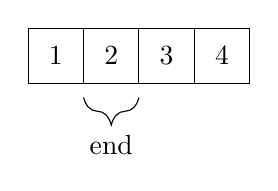
\begin{tikzpicture}[start chain = going right, node distance = 0pt, MyStyle/.style={draw, minimum width=2em, minimum height=2em, outer sep=0pt, on chain}]
	\node [MyStyle] (1) {$1$};
	\node [MyStyle] (2) {$2$};
	\node [MyStyle] (3) {$3$};
	\node [MyStyle] (4) {$4$};
	\draw[decorate,decoration={brace, amplitude=10pt, raise=5pt, mirror}] (2.south west) to node[black,midway,below= 15pt] {\code{end}} (2.south east);%
\end{tikzpicture}
\hspace{5em}
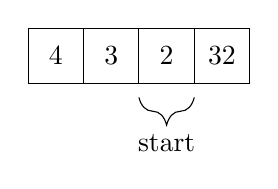
\begin{tikzpicture}[start chain = going right, node distance = 0pt, MyStyle/.style={draw, minimum width=2em, minimum height=2em, outer sep=0pt, on chain},  ]
	\node [MyStyle] (1) {$4$};
	\node [MyStyle] (2) {$3$};
	\node [MyStyle] (3) {$2$};
	\node [MyStyle] (4) {$32$};
	\draw[decorate,decoration={brace, amplitude=10pt, raise=5pt, mirror}] (3.south west) to node[black,midway,below= 15pt] {\code{start}} (3.south east);%
\end{tikzpicture}
\end{center}
\begin{center}
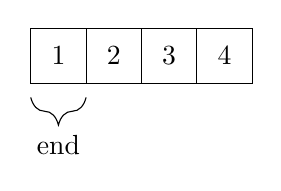
\begin{tikzpicture}[start chain = going right, node distance = 0pt, MyStyle/.style={draw, minimum width=2em, minimum height=2em, outer sep=0pt, on chain}]
	\node [MyStyle] (1) {$1$};
	\node [MyStyle] (2) {$2$};
	\node [MyStyle] (3) {$3$};
	\node [MyStyle] (4) {$4$};
	\draw[decorate,decoration={brace, amplitude=10pt, raise=5pt, mirror}] (1.south west) to node[black,midway,below= 15pt] {\code{end}} (1.south east);%
\end{tikzpicture}
\hspace{5em}
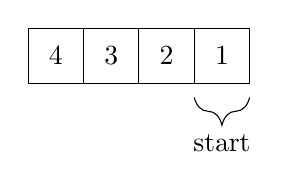
\begin{tikzpicture}[start chain = going right, node distance = 0pt, MyStyle/.style={draw, minimum width=2em, minimum height=2em, outer sep=0pt, on chain},  ]
	\node [MyStyle] (1) {$4$};
	\node [MyStyle] (2) {$3$};
	\node [MyStyle] (3) {$2$};
	\node [MyStyle] (4) {$1$};
	\draw[decorate,decoration={brace, amplitude=10pt, raise=5pt, mirror}] (4.south west) to node[black,midway,below= 15pt] {\code{start}} (4.south east);%
\end{tikzpicture}
\end{center}


	\newpage

	\subsubsection{\texttt{frequency()}}

	\lstinputlisting[language=C, firstline=110, lastline=127]{task1/task1.c}

\end{document}
